\chapter{Conclusion}\label{concChapter}

\section{Related Work}\label{concWork}

\subsection{A Language For Encoding Piece Relationships}

\citet{chessLanguage} describe a language to search across chess positions. The
main features of this language are descriptions for a chess piece
attacking/defending another, attacking/defending a square, being located at a
square, a square not being available for the enemy king, and the structure of
white/black pawns on the board.v

With their novel language, they are able to search a chess database for a
pre-determined pattern, such as the \emph{Greek gift sacrifice}, defined in the
language as `\texttt{kg8, pf7, pg7, B(ph7), Nf3, Qd1, Pe5}. With inspiration
from the FEN notation, this string corresponds to a black king on g8
(\texttt{kg8}), black pawns on f7, g7; a white bishop attacking a black pawn on
h7 (\texttt{B(ph7)}), a white knight on f3 (ready to deliver a check with
\texttt{Ng5+}, a common motif in \emph{Greek gift sacrifices}), a white queen
on d1 (\texttt{Qd1}), and finally, a white pawn on e5 (\texttt{Pe5}),
dislodging the usual black knight on f6.

This returns positions such as the one in Figure \ref{chess3}. After
\texttt{16...Be7 17. O-O}, Black blundered with \texttt{17...Bxa3??}, after
which, a \emph{Greek gift sacrifice} (\texttt{18.Bxh7!}, shown in Figure
\ref{chess4}) was made, eventually leading to a win for White.

\begin{figure}[H]
    \begin{minipage}{0.475\textwidth}
        \centering
        \chessboard[setfen=r1b2rk1/qp3ppp/p1n1pb2/4P3/3P4/P1BB1N2/5PPP/1R1QK2R
        b K - 0 16]
        \caption{\textbf{Pirc, V -- Porreca, G}, YUG-ITA m 1953, move 16.}
        \label{chess3}
    \end{minipage}
    \hspace{0.05\textwidth}
    \begin{minipage}{0.475\textwidth}
        \centering
        \chessboard[setfen=r1b2rk1/qp3ppB/p1n1p3/4P3/3P4/b1B2N2/5PPP/1R1Q1RK1 b
        - - 0 18]
        \caption{\textbf{Pirc, V -- Porreca, G}, YUG-ITA m 1953, move 18. Black
        resigned after 6 moves.}
        \label{chess4}
    \end{minipage}
\end{figure}

Their language is also able to deal with some light variations, as it is able
to identify the games shown in Figures \ref{chess5}, \ref{chess6}. In both of
these positions, White has the brilliant move \texttt{1.Qh6+!!}, following with
\texttt{2.Rh8\#} if \texttt{1...Kxh6}, and either \texttt{2.Rf7\#} or
\texttt{2.Rb7+} (leading to a quick mate) if \texttt{1...gxh6}. 

This pattern, whilst very rare, is undeniably identical between the 2 games.
The unavailability of the \texttt{g6} square to the enemy king, combined with
the harmony of White's pieces leads to the same tactic in both games.

\begin{figure}[H]
    \begin{minipage}{0.475\textwidth}
        \centering
        \chessboard[setfen=2R5/4bppk/1p1p4/5R1P/4PQ2/5P2/r4q1P/7K w - - 5 50]
        \caption{\textbf{Carlsen, M -- Karjakin S}, World Chess Championship
        2016, move 50.}
        \label{chess5}
    \end{minipage}
    \hspace{0.05\textwidth}
    \begin{minipage}{0.475\textwidth}
        \centering
        \chessboard[setfen=5R2/bp4pk/2n3p1/P7/P1q3bP/6P1/3Q3K/1R6 w - - 1 32]
        \caption{\textbf{Popov, N -- Novopashin, A}, URS-ch otbor 1979, move
        32.}
        \label{chess6}
    \end{minipage}
\end{figure}

The work of \citet{chessLanguage} is a promising proof of concept that shows
the power of a language that allows to specify piece relationships on a more
abstract level than previously possible. The biggest drawback of their
solution, as mentioned by the authors, is the fact that this language still
requires an expert with pre-existing extensive knowledge to encode the tactics
into their language.

\subsection{CQL: Chess Query Language}

The Chess Query Language (CQL), invented by \citet{cql}, is another
implementation of an advanced way to find chess positions in a given database.
Since its inception in 2004, it has grown and is able to support very powerful,
sometimes esoteric, queries to find predefined patterns.

An example of such a query is provided on the CQL website \citep{cqlSmothered},
and is shown in Figure \ref{cql} for reference. In this query, \texttt{btm}
means `black-to-move` and \texttt{mate} means checkmate is played. This
language is incredibly powerful and terse, as it allows specifying complicated
piece relationships and supports quality-of-life features such as matching
mirror positions or reversed-colour positions.

\begin{figure}[H]
    \centering
    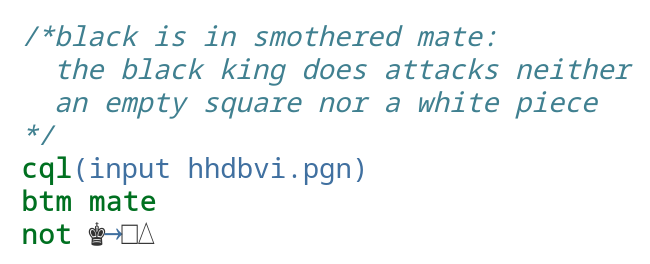
\includegraphics[width=0.45\linewidth]{background/img/cql.png}
    \caption{A CQL query to find positions where smothered mate occured.}
    \label{cql}
\end{figure}

In addition to Costeff's CQL, there exists a from-scratch clone of CQL6
\citep{cqli} which includes extra features and supports other chess variants.

\subsection{Chess Moves As Kernels For Texture Classification}

In this study, \citet{chessKernel} propose novel kernels for efficient feature
extraction in the task of texture detection. These 5x5 kernels are directly
based on the move a rook, bishop, knight, and their combinations. 

Whilst not directly applicable to the context of chess puzzle analysis, this
work shows that it may be possible to include these kernels in an CNN-based
analysis of the chess position. It would be interesting to apply to the other
CNN chess work (e.g. \citeauthor{chessCNN}'s thesis, discussed in Section
\ref{chessCNNSection}) and analyse its effect on the success of the technique.

\subsection{The Chess Transformer: Mastering Play using Generative Language
Models}\label{chessTransformerSection}

\citet{chessTransformer} demonstrate the ability of transformers to learn the
rules of chess and complex gameplay by analysing PGN games with a fine-tuned
GPT-2 transformer. By treating PGN games as a sequence of natural language
words, the authors show successful results and are able to generate new games
without specifying chess rules.

A key downside of their work is that their model generates illegal moves, which
have to be filtered manually using a chess library \citep{chessTransformer}.
This `hallucination' effect is a downside of using transformers, and other
generative techniques, in chess. 

